\documentclass[aspectratio=169,11pt]{beamer}

\usepackage[utf8]{inputenc}
\usepackage[T1]{fontenc}
\usepackage[french]{babel}
\usepackage{lmodern}
\usepackage{graphicx}
\usepackage{booktabs}
\usepackage{tikz}
\usetikzlibrary{positioning,arrows.meta}

\definecolor{condruBlue}{RGB}{20,82,112}
\definecolor{condruGreen}{RGB}{64,128,91}
\definecolor{condruRed}{RGB}{204,57,57}
\definecolor{condruInk}{RGB}{30,38,44}
\definecolor{condruSoft}{RGB}{244,247,246}

\usetheme{Madrid}
\usecolortheme{default}
\setbeamertemplate{navigation symbols}{}
\setbeamertemplate{footline}{}
\setbeamertemplate{itemize item}{\color{condruGreen}$\blacktriangleright$}
\setbeamertemplate{itemize subitem}{\color{condruBlue}$\bullet$}
\setbeamercolor{title}{fg=white,bg=condruBlue}
\setbeamercolor{frametitle}{fg=white,bg=condruBlue}
\setbeamercolor{structure}{fg=condruBlue}
\setbeamercolor{block title}{fg=white,bg=condruBlue}
\setbeamercolor{block body}{fg=condruInk,bg=condruSoft}
\setbeamerfont{frametitle}{series=\bfseries}

\title[CondruLytics]{CondruLytics}
\subtitle{Analyse, prédiction et visualisation des résultats \\ du Challenge Condrusien \\ de 2006 à 2025}
\author{Michaël Mestré}
\institute{Université de Namur -- Faculté d'Informatique}
\date{Juin 2026}

\newcommand{\metric}[2]{%
  \begin{minipage}{0.22\textwidth}
    \centering
    {\Large\bfseries\color{condruBlue} #1}\\[-1mm]
    {\scriptsize #2}
  \end{minipage}
}

\newcommand{\bigmessage}[1]{%
  \begin{center}
    \vspace{0.7cm}
    {\Large\bfseries\color{condruBlue} #1}
    \vspace{0.4cm}
  \end{center}
}

\begin{document}

\begin{frame}
  \titlepage
  \vspace{-0.8cm}
  \begin{center}
    
\includegraphics[height=1.2cm]{unamur.png}
  \end{center}
\end{frame}

% Attention getter
\begin{frame}{Le Challenge Condrusien}
  \begin{columns}[T,onlytextwidth]
    \begin{column}{0.52\textwidth}
      \begin{block}{Contexte}
        \begin{itemize}
          \item Challenge de course à pied amateur dans le Condroz liégeois.
          \item Environ une vingtaine d'organisations par saison.
          \item Plusieurs formats : petite distance, grande distance, parfois trail.
          \item Des classements publiés après chaque course.
        \end{itemize}
      \end{block}
      \vspace{0.2cm}
    \end{column}
    \begin{column}{0.44\textwidth}
      \centering
      
\includegraphics[height=0.5\textheight]{logo.png}
    \end{column}
  \end{columns}
  \begin{center}
        {\large\bfseries\color{condruBlue}
        Chaque résultat est lisible, mais sa comparaison est difficile.}
      \end{center}
\end{frame}

% Need
\begin{frame}{Besoin : comparer des performances}
  \begin{columns}[T,onlytextwidth]
    \begin{column}{0.52\textwidth}
      Les classements sont consultables, mais ils répondent mal aux questions d'un coureur.
      \vspace{0.3cm}
      \begin{itemize}
        \item Ai-je progressé, ou la course était-elle plus facile ?
        \item Comment comparer un 6 km roulant sur route et un 12 km vallonné sur chemin ?
        \item Ai-je mieux couru que d'habitude par rapport aux autres ?
        \item Quel temps aurais-je pu faire sur une course non courue ?
      \end{itemize}
    \end{column}
    \begin{column}{0.44\textwidth}
      \begin{block}{Besoin}
        Passer d'une lecture de classement à une lecture comparative, personnelle et contextualisée.
      \end{block}
      \vspace{0.35cm}
      \centering
      {\Large Classement}\\[0.15cm]
      {\color{condruGreen}\Large $\downarrow$}\\[0.15cm]
      {\Large Indicateur comparable}\\[0.15cm]
      {\color{condruGreen}\Large $\downarrow$}\\[0.15cm]
      {\Large Analyse coureur}
    \end{column}
  \end{columns}
\end{frame}

% Main message
\begin{frame}{}
  \begin{center}
    \vspace{0.8cm}
    {\huge\bfseries\color{condruBlue} CondruLytics}\\[0.5cm]
    {\Large transforme des classements historiques en}\\[0.2cm]
    {\Large\bfseries données structurées, indicateurs de performance et simulations interprétables.}
  \end{center}
\end{frame}

% Preview
\begin{frame}{Agenda}
  \begin{enumerate}
    \item Données de départ
    \item Pipeline ETL
    \item Nettoyage et correction des coureurs
    \item Chargement PostgreSQL et modèle relationnel
    \item Feature engineering et prédiction
    \item Application Streamlit et démonstration
    \item Conclusion, limites et perspectives
  \end{enumerate}
\end{frame}

\section{Données et pipeline}

\begin{frame}{Données disponibles (2006-2025)}
  \begin{center}
    \metric{588}{fichiers PDF}
    \metric{114\,761}{résultats nettoyés}
    \metric{566}{courses}
    \metric{24\,264}{noms normalisés}
  \end{center}
  \vspace{0.7cm}
  \begin{block}{}
    Le volume est raisonnable, mais la difficulté vient de l'hétérogénéité des fichiers disponibles, de la qualité des extractions et des corrections.
  \end{block}
\end{frame}

\begin{frame}{Pipeline général}
  \centering
  \resizebox{0.95\textwidth}{!}{%
  \begin{tikzpicture}[
    flowbox/.style={draw, rounded corners=2pt, fill=condruSoft, align=center,
      text width=2.8cm, minimum height=1.15cm, font=\small},
    db/.style={draw=condruBlue, rounded corners=2pt, fill=blue!8, align=center,
      text width=2.8cm, minimum height=1.15cm, font=\small},
    model/.style={draw=condruGreen, rounded corners=2pt, fill=green!8, align=center,
      text width=2.8cm, minimum height=1.15cm, font=\small},
    arrow/.style={-{Latex[length=3mm]}, thick, color=condruInk}
  ]
    \node[flowbox] (zip) {Archives ZIP\\et PDF};
    \node[flowbox, right=0.6cm of zip] (parse) {Parsing\\spécialisé};
    \node[flowbox, right=0.6cm of parse] (clean) {Nettoyage\\harmonisation};
    \node[db, right=0.6cm of clean] (db) {Base\\PostgreSQL};
    \node[model, below=1.1cm of db] (feat) {Feature\\engineering};
    \node[model, left=0.6cm of feat] (pred) {Régression\\z-score};
    \node[flowbox, left=0.6cm of pred] (app) {Application\\Streamlit};

    \draw[arrow] (zip) -- (parse);
    \draw[arrow] (parse) -- (clean);
    \draw[arrow] (clean) -- (db);
    \draw[arrow] (db) -- (feat);
    \draw[arrow] (feat) -- (pred);
    \draw[arrow] (pred) -- (app);
    \draw[arrow] (db.south west) -- ++(0,-0.55) -| (app.north);
  \end{tikzpicture}}
\end{frame}

\begin{frame}{Parsing : plusieurs stratégies selon les années}
  \begin{columns}[T,onlytextwidth]
    \begin{column}{0.49\textwidth}
      \centering
      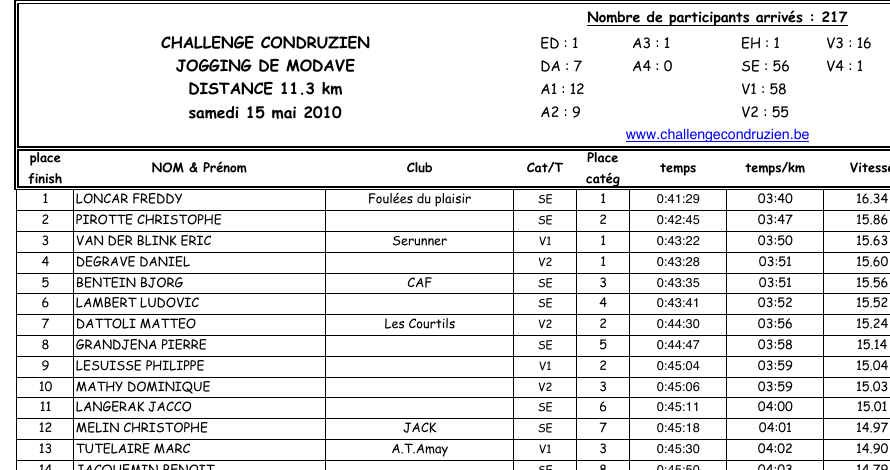
\includegraphics[width=\linewidth,height=0.34\textheight,keepaspectratio]{pdf_format_2010.png}
    \end{column}
    \begin{column}{0.49\textwidth}
      \centering
      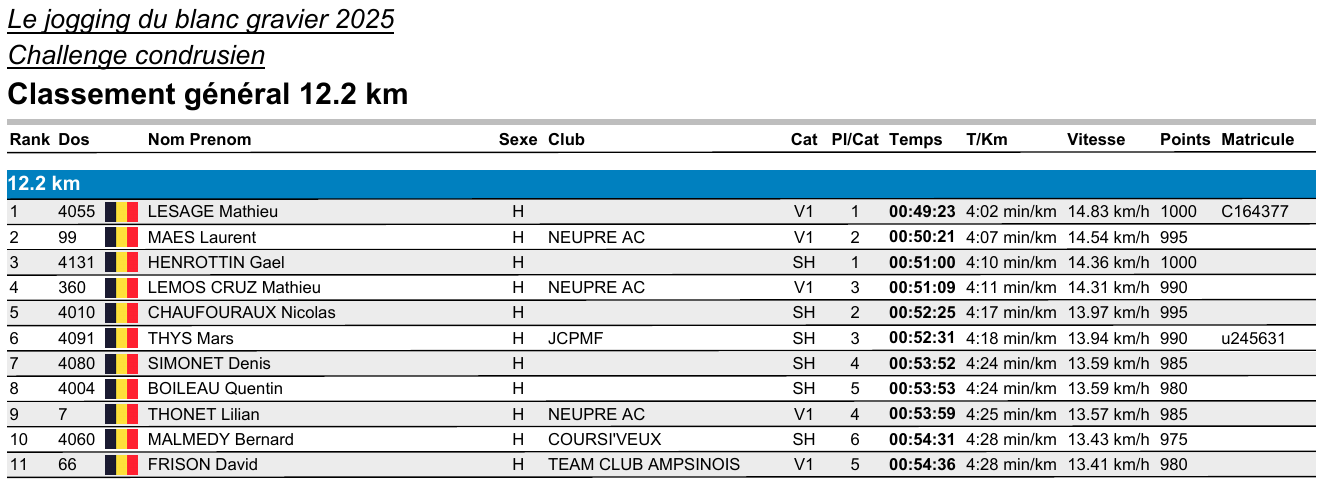
\includegraphics[width=\linewidth,height=0.34\textheight,keepaspectratio]{pdf_format_2025.png}
    \end{column}
  \end{columns}

  \vspace{0.1cm}
  \begin{columns}[T,onlytextwidth]
    \begin{column}{0.52\textwidth}
      \begin{itemize}
        \item \texttt{Parser2006\_2007}
        \item \texttt{Parser2008\_2016}
        \item \texttt{Parser2017\_2024}
        \item \texttt{Parser2025}
      \end{itemize}
    \end{column}
    \begin{column}{0.44\textwidth}
      \begin{block}{Choix d'implémentation}
        Un \textit{ParserFactory} sélectionne automatiquement la stratégie adaptée au fichier analysé.
      \end{block}
    \end{column}
  \end{columns}
  \vspace{0.1cm}
  \centering
  {\small Chaque fichier est converti en données tabulaires puis sauvegardé en Parquet.}
\end{frame}

\section{Nettoyage}

\begin{frame}{Correction des noms de coureurs}
  \begin{columns}[T,onlytextwidth]
    \begin{column}{0.48\textwidth}
      \begin{block}{Problème}
        Une même personne peut apparaître avec plusieurs variantes de nom.
      \end{block}
      \begin{itemize}
        \item accents, tirets, apostrophes ;
        \item fautes de frappe ;
        \item bruit d'extraction PDF ;
        \item homonymes possibles.
      \end{itemize}
    \end{column}
    \begin{column}{0.48\textwidth}
      \begin{block}{Correction prudente}
         Accepter seulement les rapprochements à confiance élevée.
      \end{block}
      \begin{itemize}
        \item similarité de nom (fuzzy matching) ;
        \item sexe compatible ;
        \item vitesse moyenne cohérente ;
        \item pas de doublon sur une même course.
      \end{itemize}
    \end{column}
  \end{columns}
\end{frame}

\section{Base de données}

\begin{frame}{Base de données : résultats observés}
  \centering
  \resizebox{0.92\textwidth}{!}{%
  \begin{tikzpicture}[
    dim/.style={draw, rounded corners=2pt, fill=condruSoft, align=left,
      text width=3.6cm, minimum height=2.2cm, font=\small, inner sep=7pt},
    fact/.style={draw=condruBlue, rounded corners=2pt, fill=blue!8, align=left,
      text width=4.1cm, minimum height=2.5cm, font=\small, inner sep=7pt},
    arrow/.style={-{Latex[length=3mm]}, thick, color=condruInk}
  ]
    \node[fact] (fact) {
      \textbf{fact\_results}\\
      \rule{\linewidth}{0.3pt}\\
      result\_id\\
      runner\_id, race\_id\\
      position\\
      time\_sec, speed\_kmh\\
      category\_clean
    };

    \node[dim, left=1.8cm of fact] (runner) {
      \textbf{dim\_runner}\\
      \rule{\linewidth}{0.3pt}\\
      runner\_id\\
      name\_origin\\
      name\_clean\\
      sex
    };

    \node[dim, right=1.8cm of fact] (race) {
      \textbf{dim\_race}\\
      \rule{\linewidth}{0.3pt}\\
      race\_id\\
      racekey\\
      name\\
      distance\\
      date, year
    };

    \draw[arrow] (fact.west) -- (runner.east);
    \draw[arrow] (fact.east) -- (race.west);
  \end{tikzpicture}}
  \vspace{0.3cm}
  \begin{block}{Granularité}
    Une ligne de \texttt{fact\_results} correspond à un résultat observé : un coureur sur une course.
  \end{block}
  \begin{block}{Choix technique}
        \begin{itemize}
          \item PostgreSQL lancé via Docker ;
          \item chargement avec SQLAlchemy ;
        \end{itemize}
      \end{block}
\end{frame}

\begin{frame}{Base de données : feature engineering et prédiction}
  \centering
  \resizebox{0.94\textwidth}{!}{%
    \begin{tikzpicture}[
        dim/.style={draw, rounded corners, align=left, text width=3.2cm, minimum height=1.6cm, fill=gray!8, font=\small},
        analytic/.style={draw, rounded corners, align=left, text width=10.8cm, fill=green!8, inner sep=8pt, font=\scriptsize},
        link/.style={-{Latex[length=3mm]}, thick}
    ]
        \node[analytic] (analysis) {
            \textbf{fact\_runner\_race\_analysis}\\
            \rule{\linewidth}{0.3pt}\\
            \setlength{\tabcolsep}{2pt}
            \begin{tabular}{@{}p{3.85cm}p{3.1cm}p{3.2cm}@{}}
              \texttt{analysis\_id} (PK) &
              race\_month &
              prior\_race\_count \\
              \texttt{source\_result\_id} &
              race\_dayofyear &
              prior\_avg\_speed \\
              \texttt{runner\_id} (FK) &
              race\_participants &
              prior\_std\_speed \\
              \texttt{race\_id} (FK) &
              race\_mean\_speed &
              prior\_best\_speed \\
              actual\_position &
              race\_std\_speed &
              prior\_avg\_z \\
              actual\_position\_category &
              race\_median\_speed &
              prior\_std\_z \\
              actual\_time\_sec &
              speed\_z\_race &
              prior\_best\_z \\
              actual\_speed\_kmh &
              performance\_index &
              recent\_speed\_roll3 \\
              target\_z &
              split &
              recent\_z\_roll3 \\
              predicted\_z &
              &
              days\_since\_last\_race \\
              predicted\_performance\_index &
              &
              runner\_history\_years \\
              predicted\_speed\_kmh &
              &
              predicted\_time\_sec \\
              abs\_error\_time\_sec &
              &
              \\
            \end{tabular}
        };

        \node[dim, right=1.1cm of analysis.north east, anchor=north west] (runner) {
            \textbf{dim\_runner}\\
            \rule{\linewidth}{0.3pt}\\
            \texttt{runner\_id} (PK)\\
            ...
        };

        \node[dim, below=0.7cm of runner] (race) {
            \textbf{dim\_race}\\
            \rule{\linewidth}{0.3pt}\\
            \texttt{race\_id} (PK)\\
            ...
        };

        \draw[link] (analysis.east) -- (runner.west);
        \draw[link] (analysis.east) -- (race.west);
    \end{tikzpicture}}
\end{frame}

\section{Modélisation}

\begin{frame}{Indice de performance : normalisation par course}
  \begin{columns}[T,onlytextwidth]
    \begin{column}{0.52\textwidth}
      \begin{block}{Même coureur, contextes différents}
        Une allure brute ne suffit pas pour comparer deux courses.
      \end{block}
      \begin{itemize}
        \item Le dénivelé peut ralentir une course.
        \item La nature du sol change l'effort réel.
        \item La météo peut modifier fortement le résultat.
      \end{itemize}
    \end{column}
    \begin{column}{0.44\textwidth}
      \begin{center}
        {\Large\bfseries\color{condruBlue}
        $z = \frac{v - \mu_{\mathrm{course}}}{\sigma_{\mathrm{course}}}$}\\[0.5cm]
        {\large Indice = $100 + 10z$}
      \end{center}
      \begin{block}{Idée}
        Comparer le coureur aux participants de la même course, qui partagent globalement les mêmes conditions.
      \end{block}
    \end{column}
  \end{columns}
\end{frame}

\begin{frame}{Prédiction du temps de course : régression sur le z-score}
  \begin{block}{Objectif}
    Estimer le temps qu'un coureur aurait pu faire sur une course non courue.
  \end{block}

  \vspace{0.2cm}
  \begin{columns}[T,onlytextwidth]
    \begin{column}{0.42\textwidth}
      \begin{block}{Modèle}
      \begin{itemize}
        \item Régression linéaire sur z-score ;
        \item Variables explicatives issues de l'historique du coureur et du contexte de la course ;
        \item Découpage temporel : entraînement sur les années passées, test sur 2025.
      \end{itemize}
      \end{block}
    \end{column}

    \begin{column}{0.54\textwidth}
      \begin{block}{Conversion en vitesse prédite}
        \small
        \[
        \begin{aligned}
        vitesse\_predite &= \\
        &\quad moyenne\_course \\
        &\quad + z\_predit \times ecart\_type\_course
        \end{aligned}
        \]
      \end{block}

      \vspace{0.15cm}
      \begin{block}{Conversion en temps prédit}
        \small
        \[
        \begin{aligned}
        temps\_predit &= \\
        &\quad \frac{distance}{vitesse\_predite} \times 3600
        \end{aligned}
        \]
      \end{block}
    \end{column}
  \end{columns}
\end{frame}

\begin{frame}{Résultats de la régression}
  \begin{center}
    \begin{tabular}{lrrrr}
      \toprule
      Jeu & n & MAE z & $R^2$ z & MAE temps \\
      \midrule
      Entraînement & 74\,589 & 0,331 & 0,771 & 217 s \\
      Test 2025 & 5\,627 & 0,335 & 0,778 & 200 s \\
      \bottomrule
    \end{tabular}
  \end{center}
  \vspace{0.5cm}
  \begin{block}{Interprétation}
    Le modèle capte une tendance générale sans surapprentissage évident, mais la prédiction reste une aide à l'analyse plutôt qu'une vérité sportive.
  \end{block}
\end{frame}

\begin{frame}{Temps réel vs temps prédit}
  \centering
  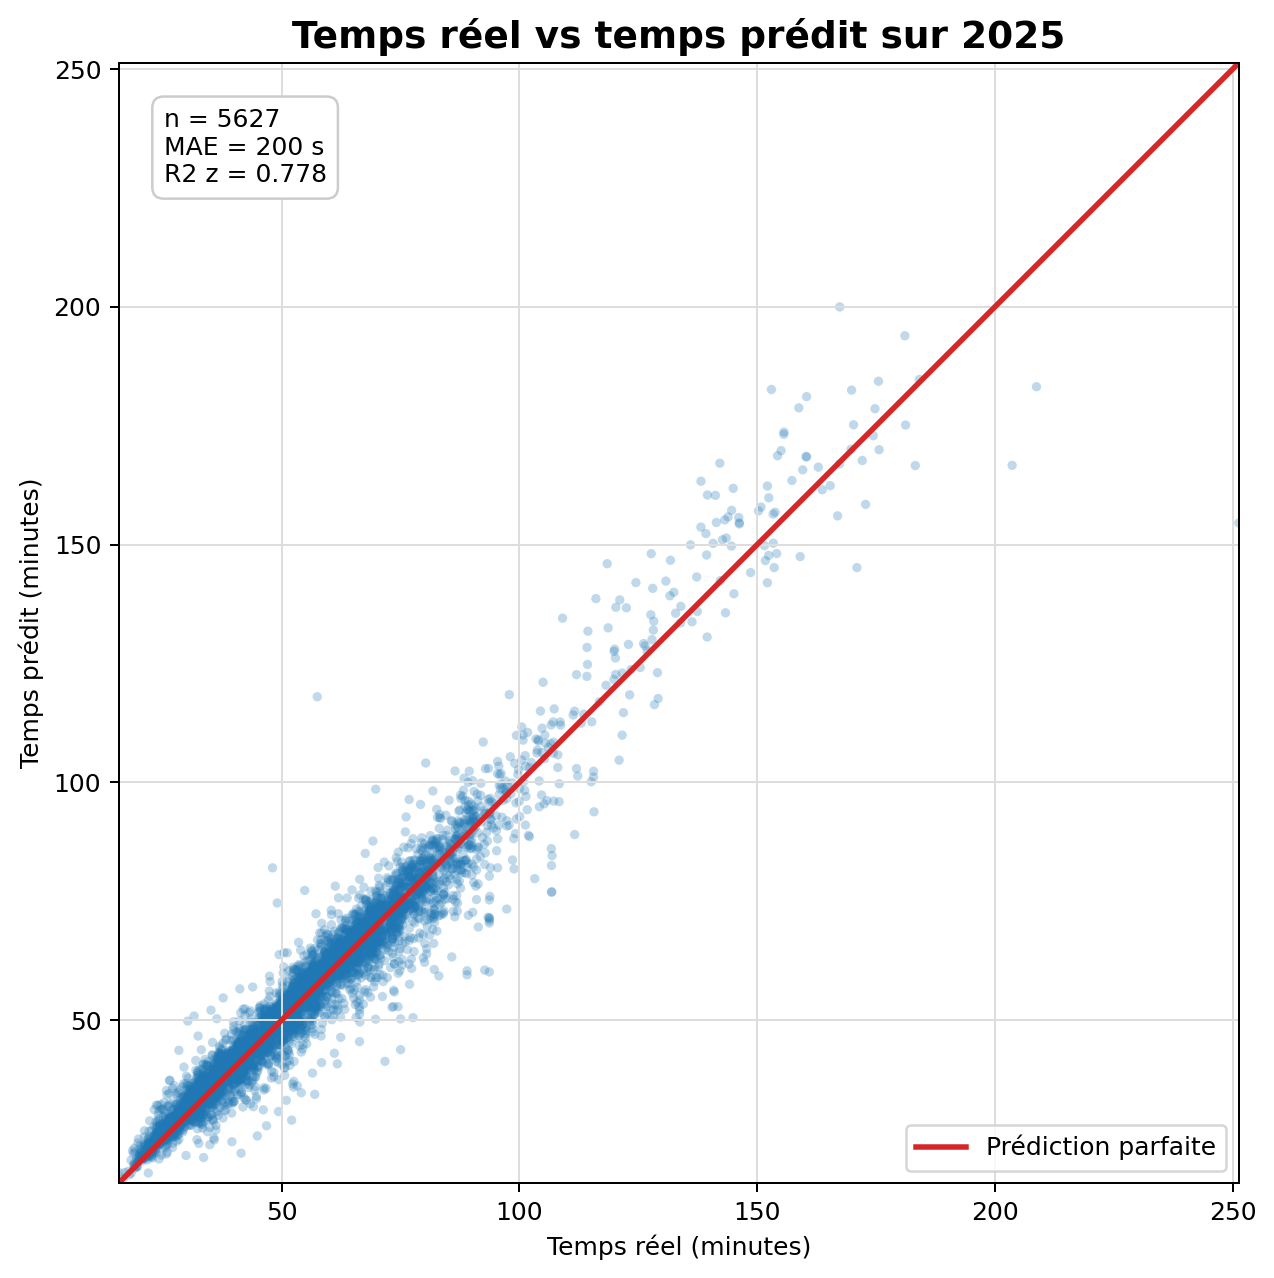
\includegraphics[height=0.78\textheight]{temps_reel_vs_predit_2025.png}
\end{frame}

\begin{frame}{Variables les plus influentes}
  \begin{columns}[T,onlytextwidth]
    \begin{column}{0.56\textwidth}
      \begin{center}
        \small
        \begin{tabular}{lrr}
          \toprule
          Variable & Coef. & $|$Coef.$|$ \\
          \midrule
          recent\_z\_roll3 & 0,5118 & 0,5118 \\
          prior\_avg\_speed & 0,2894 & 0,2894 \\
          distance & -0,1387 & 0,1387 \\
          prior\_avg\_z & 0,1055 & 0,1055 \\
          race\_month & -0,0549 & 0,0549 \\
          recent\_speed\_roll3 & 0,0542 & 0,0542 \\
          prior\_std\_z & 0,0410 & 0,0410 \\
          prior\_best\_z & -0,0381 & 0,0381 \\
          \bottomrule
        \end{tabular}
      \end{center}
    \end{column}

    \begin{column}{0.4\textwidth}
      \begin{block}{}
        Le modèle s'appuie surtout sur la forme récente du coureur et son niveau moyen historique.
      \end{block}
    \end{column}
  \end{columns}
\end{frame}



\section{Personas et application}

\begin{frame}{Personas : deux usages complémentaires}
  \begin{columns}[T,onlytextwidth]
    \begin{column}{0.48\textwidth}
      \begin{block}{Claire, coureuse loisir}
        \begin{itemize}
          \item Comprendre ses résultats sans vocabulaire statistique.
          \item Savoir si elle progresse au fil des courses.
          \item Identifier les courses où elle a mieux couru que d'habitude.
        \end{itemize}
      \end{block}
    \end{column}
    \begin{column}{0.48\textwidth}
      \begin{block}{Marc, coureur régulier}
        \begin{itemize}
          \item Comparer ses performances entre distances.
          \item Se situer par rapport aux autres coureurs.
          \item Estimer un temps probable sur une course non courue.
        \end{itemize}
      \end{block}
    \end{column}
  \end{columns}
  \vspace{0.4cm}
  \bigmessage{L'application doit transformer les classements en réponses actionnables.}
\end{frame}

\begin{frame}{Démonstration live}

    \begin{enumerate}
      \item Vue d'ensemble : période, courses et volume de résultats.
      \item Vue course : classement, catégories, temps attendu.
      \item Vue coureur : évolution de l'indice de performance.
      \item Simulation : temps estimé sur une course non courue.
    \end{enumerate}

  \vspace{0.5cm}
\end{frame}

\section{Conclusion}

\begin{frame}{Conclusions}
      \begin{itemize}
        \item Les PDF historiques ont été structurés.
        \item Les noms, courses, temps et catégories ont été harmonisés.
        \item Un indice de performance rend les courses comparables.
        \item L'application permet l'exploration et la simulation.
      \end{itemize}
\end{frame}



\begin{frame}{Limites et perspectives}
  \begin{center}
    \renewcommand{\arraystretch}{1.7}
    \begin{tabular}{p{0.25\textwidth}p{0.29\textwidth}p{0.29\textwidth}}
      \toprule
      & \textbf{Limite} & \textbf{Perspective} \\
      \midrule
      \textbf{Données} &
      PDF hétérogènes &
      Tests automatisés \\
      \textbf{Coureurs} &
      Identification par le nom &
      Matching robuste \\
      \textbf{Modèle} &
      Simulation rétrospective &
      Courses futures et données parcours \\
      \bottomrule
    \end{tabular}
  \end{center}
\end{frame}

\begin{frame}{}
  \begin{center}
    {\Large\bfseries\color{condruBlue}
    CondruLytics rend visible l'histoire sportive du \\ Challenge Condrusien.}\\[0.5cm]
  \end{center}
\end{frame}



\appendix
\section{Backup}

\begin{frame}[noframenumbering]{Backup : vue d'ensemble}
  \centering
  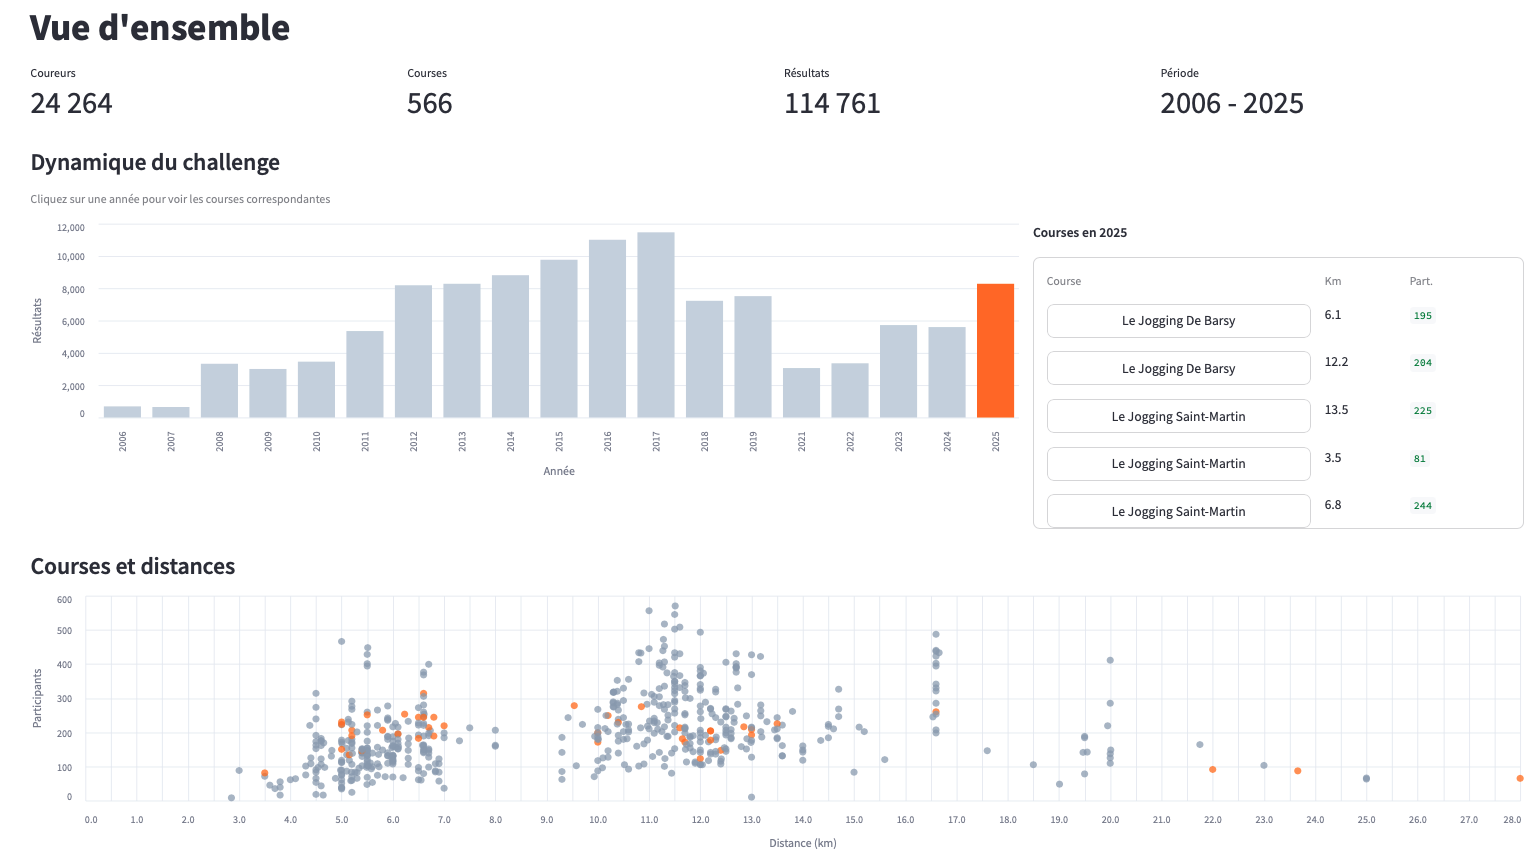
\includegraphics[height=0.74\textheight,keepaspectratio]{vue_ensemble.png}
\end{frame}

\begin{frame}[noframenumbering]{Backup : vue course}
  \centering
  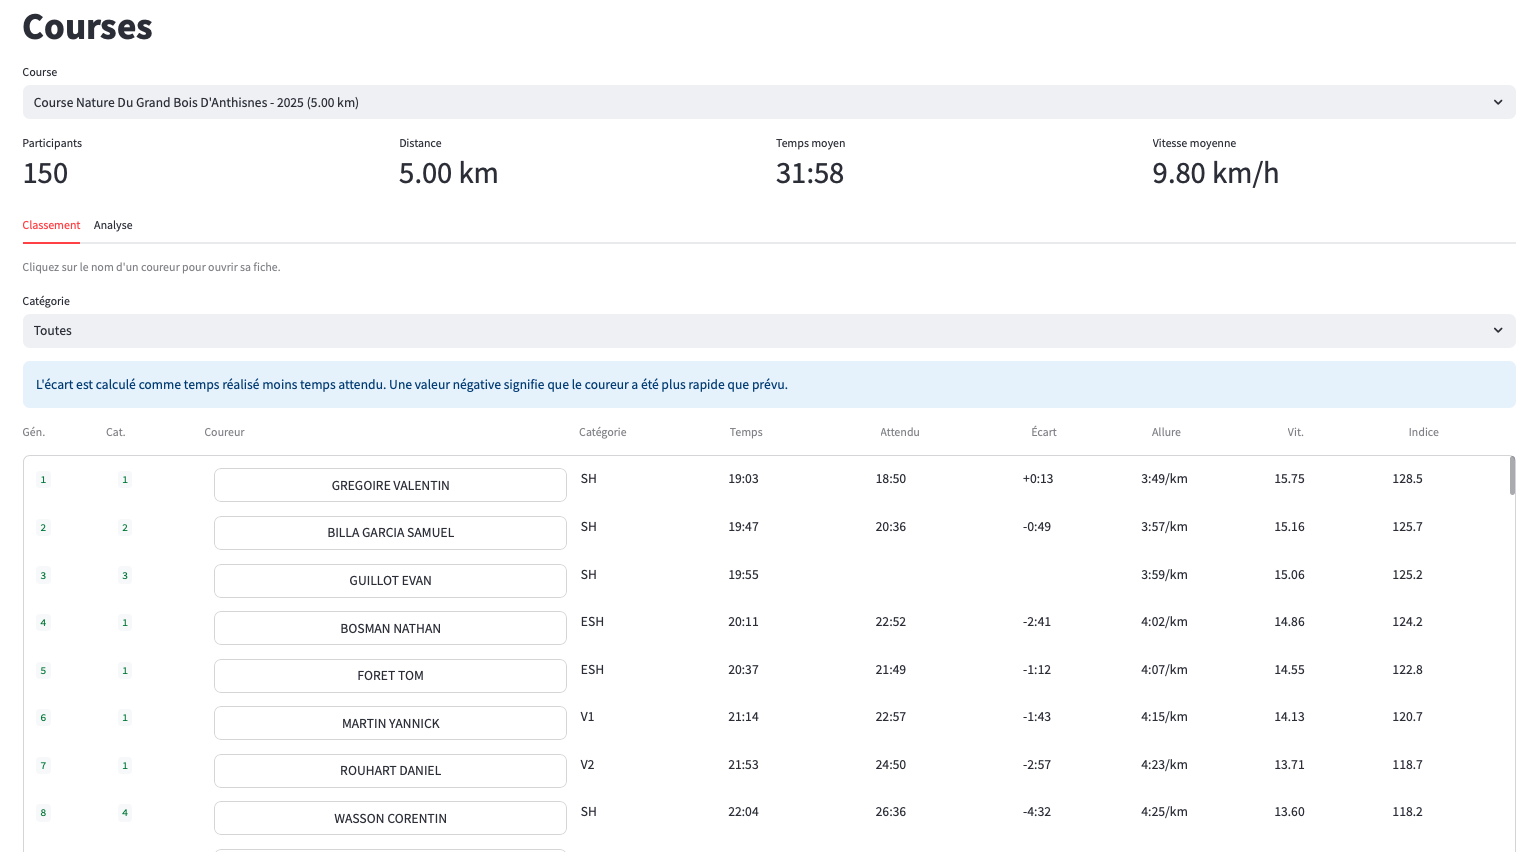
\includegraphics[height=0.74\textheight,keepaspectratio]{course_classement.png}
\end{frame}

\begin{frame}[noframenumbering]{Backup : vue coureur}
  \centering
  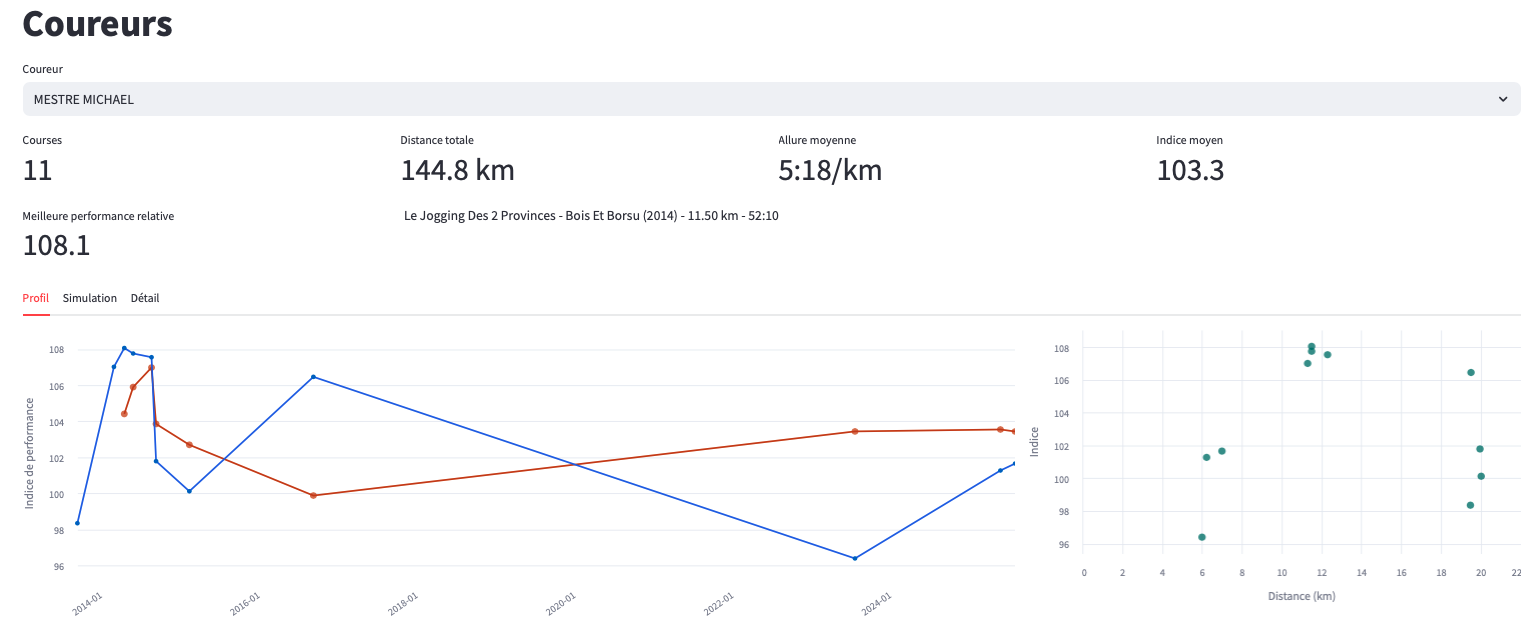
\includegraphics[height=0.74\textheight,keepaspectratio]{coureur_profil.png}
\end{frame}

\begin{frame}[noframenumbering]{Backup : simulation rétrospective}
  \centering
  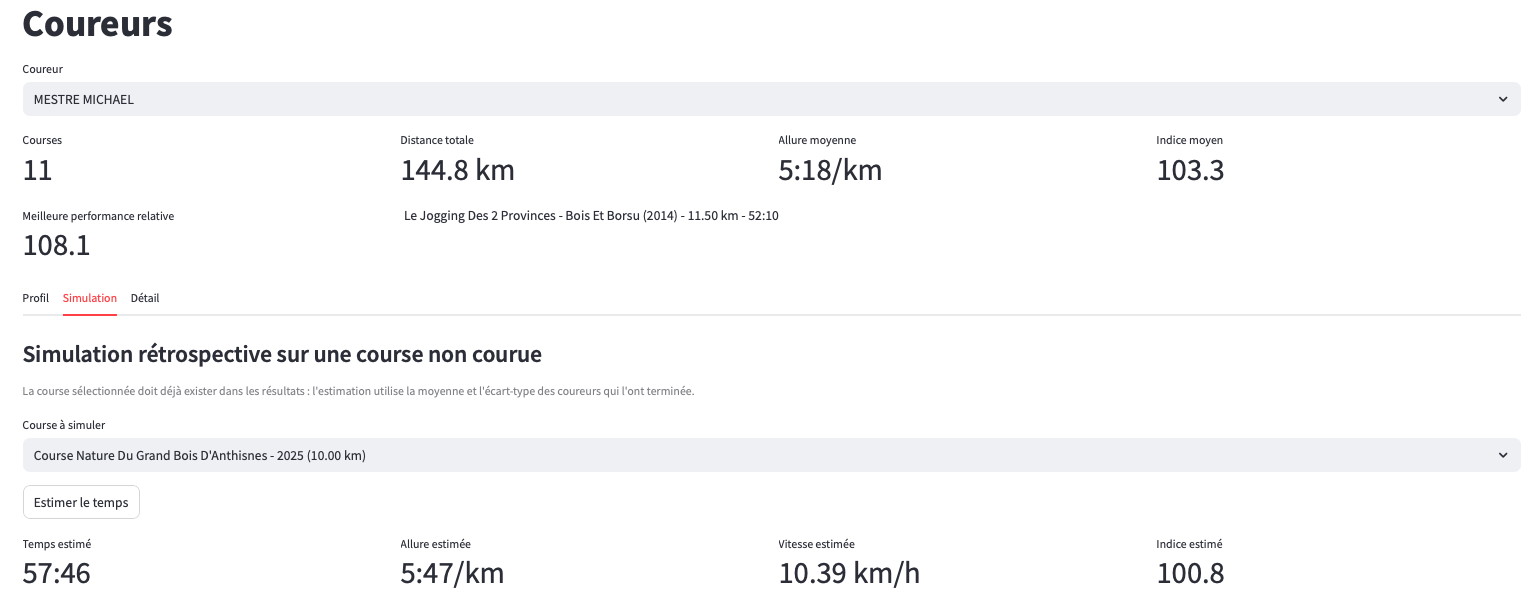
\includegraphics[height=0.74\textheight,keepaspectratio]{coureur_simulation.png}
\end{frame}

\end{document}
